\documentclass[a4paper,journal]{IEEEtran}

\usepackage{amsmath,amssymb,amsfonts}
\usepackage{booktabs}
\usepackage{fancyhdr}
\usepackage{graphicx}
\usepackage[hidelinks,hypertexnames=false]{hyperref}
\usepackage{pdfpages}

\graphicspath{{media/}}

\setlength{\headheight}{14.5pt}
\fancypagestyle{portfolioappendix}{%
    \fancyhf{}%
    \fancyhead[R]{\thepage}%
    \renewcommand{\headrulewidth}{0pt}%
    \renewcommand{\footrulewidth}{0pt}%
}

\newcommand{\PortfolioImportedPageCommand}{%
    \thispagestyle{portfolioappendix}%
}
\newcommand{\PortfolioAppendixPageStyle}{%
    \pagestyle{portfolioappendix}%
}
\newcommand{\PortfolioContentPageCommand}{%
    \thispagestyle{portfolioappendix}%
}
% Imported PDF entries already carry their paper/appendix identifiers in the
% supplied title. Suppress IEEEtran's additional I-A/D-J prefixes in Contents.
\makeatletter
\renewcommand{\AM@addtotoc@hook}{%
    \def\thesection{}%
    \def\thesubsection{}%
    \def\@IEEEsectpunct{}%
}
\makeatother
\newcommand{\PortfolioAppendixTitle}[2]{%
    \onecolumn
    \thispagestyle{empty}
    \centering
    \vspace*{0.34\textheight}
    {\fontsize{24}{29}\selectfont\bfseries Appendix #1\par}
    \vspace{1.5em}
    {\fontsize{24}{29}\selectfont\bfseries #2\par}
    \clearpage
}
\newcommand{\StartAppendixPages}[1]{%
    \renewcommand{\thepage}{#1.\arabic{page}}%
    \setcounter{page}{1}%
    \pagestyle{portfolioappendix}%
}

\begin{document}
\onecolumn
\pagenumbering{gobble}
\makeatletter
\renewcommand{\@pnumwidth}{3em}
\makeatother

\begin{titlepage}
    \thispagestyle{empty}
    \centering
    \vspace*{0.22\textheight}
    {\fontsize{24}{29}\selectfont\bfseries
      Using Machine Learning to Predict Scattering Parameters\par
      for Signal Integrity Purposes\par}
    \vspace{2.2em}
    {\fontsize{24}{29}\selectfont\bfseries Project Portfolio\par}
    \vfill
    {\large Chunyu Long\par}
    \vspace{0.5em}
    {\large Student ID: A00049113\par}
    \vspace{1.5em}
    {\large Supervisor: Dr Marissa Condon\par}
    \vspace{1.5em}
    {\large August 2026\par}
    \vspace*{0.08\textheight}
\end{titlepage}

\section*{Acknowledgements}
I would like to thank my supervisor, Dr Marissa Condon, for her guidance
throughout this project. I also acknowledge the authors and maintainers of the
SI/PI-Database for making the simulated PCB-interconnect data available for
research.

\clearpage
\tableofcontents

\clearpage
\pagenumbering{arabic}
\setcounter{page}{1}
\includepdf[
    pages=-,
    fitpaper=true,
    pagecommand={\thispagestyle{empty}},
    addtotoc={
        1,section,1,{Research Paper},paper:main,
        1,subsection,2,{Abstract, Introduction and Prior Work},paper:page-one,
        2,subsection,2,{Dataset and Methodology},paper:methodology,
        4,subsection,2,{Experimental Results},paper:results,
        5,subsection,2,{Analysis and Discussion},paper:analysis,
        6,subsection,2,{Conclusion and References},paper:conclusion
    }
]{build/A00049113_EEN1095_Research_Paper.pdf}

\PortfolioAppendixTitle{A}{Use of GenAI}
\StartAppendixPages{A}
\addcontentsline{toc}{section}{Appendix A --- Use of GenAI}
% !TEX root = ../main.tex
% Appendix A source fragment. Do not input this file into the six-page paper.
% The overall portfolio wrapper must load booktabs and pdfpages, create the
% Appendix A title page, establish A.1/A.2/... pagination and define the
% optional imported-page hook below.
\providecommand{\PortfolioImportedPageCommand}{}

\phantomsection
\addcontentsline{toc}{subsection}{A.1 Summary of GenAI Use}
\subsection*{A.1 Summary of GenAI Use}
\label{app:a-summary}

Generative artificial intelligence (GenAI) tools were used as drafting and
documentation aids during the project. They did not generate the simulation
dataset or replace the reported model training and evaluation. Table~
\ref{tab:appendix-a-summary} identifies the use recorded in the current
cumulative log, its benefit and the parts of the project that it informed.

\begin{table}[htbp]
    \caption{GenAI use recorded in the current cumulative log.}
    \label{tab:appendix-a-summary}
    \centering
    \scriptsize
    \begin{tabular}{@{}p{0.14\textwidth}p{0.25\textwidth}
                         p{0.25\textwidth}p{0.25\textwidth}@{}}
        \toprule
        Tool and period & Purpose and benefit & Material informed
          & Review and limitations \\
        \midrule
        Claude Code,
        Weeks 7--10
          & Summarised Git history and helped organise development-log
            material, saving time when tracing changes across files and
            commits.
          & Bi-weekly development records later consulted when preparing the
            progress and milestone account in Appendix C.
          & The summaries were checked against commits and project files.
            Work outside version control and experimental quality still
            required manual review. \\
        Gemini,
        Week 11--12
          & Drafted a progress summary and helped interpret milestone status
            consistently.
          & The Week 11--12 development record and the progress/status account
            consolidated in Appendix C.
          & Dates, milestones and implementation claims were checked against
            the repository and approved project plan. \\
        Gemini Notebook
        (NotebookLM),
        Week 13--14
          & Condensed the project narrative, organised prior work into themes
            and produced an initial LaTeX design-variable table.
          & The paper's Abstract, Introduction, Prior Work discussion and
            Table I in Section III.
          & Claims were checked against primary papers, executed notebooks and
            saved metrics. Unsupported statements, including claims that
            passivity and causality were enforced, were corrected. \\
        \bottomrule
    \end{tabular}
\end{table}

The tools were used to propose summaries, structure and wording. Experimental
values in the paper and appendices were taken from executed notebooks and saved
artifacts, then independently reproduced in Notebook 07. Literature claims were
checked against the cited sources. Generated text was revised for accuracy,
scope and consistency with the completed work. The author remains responsible
for the final content.

\clearpage
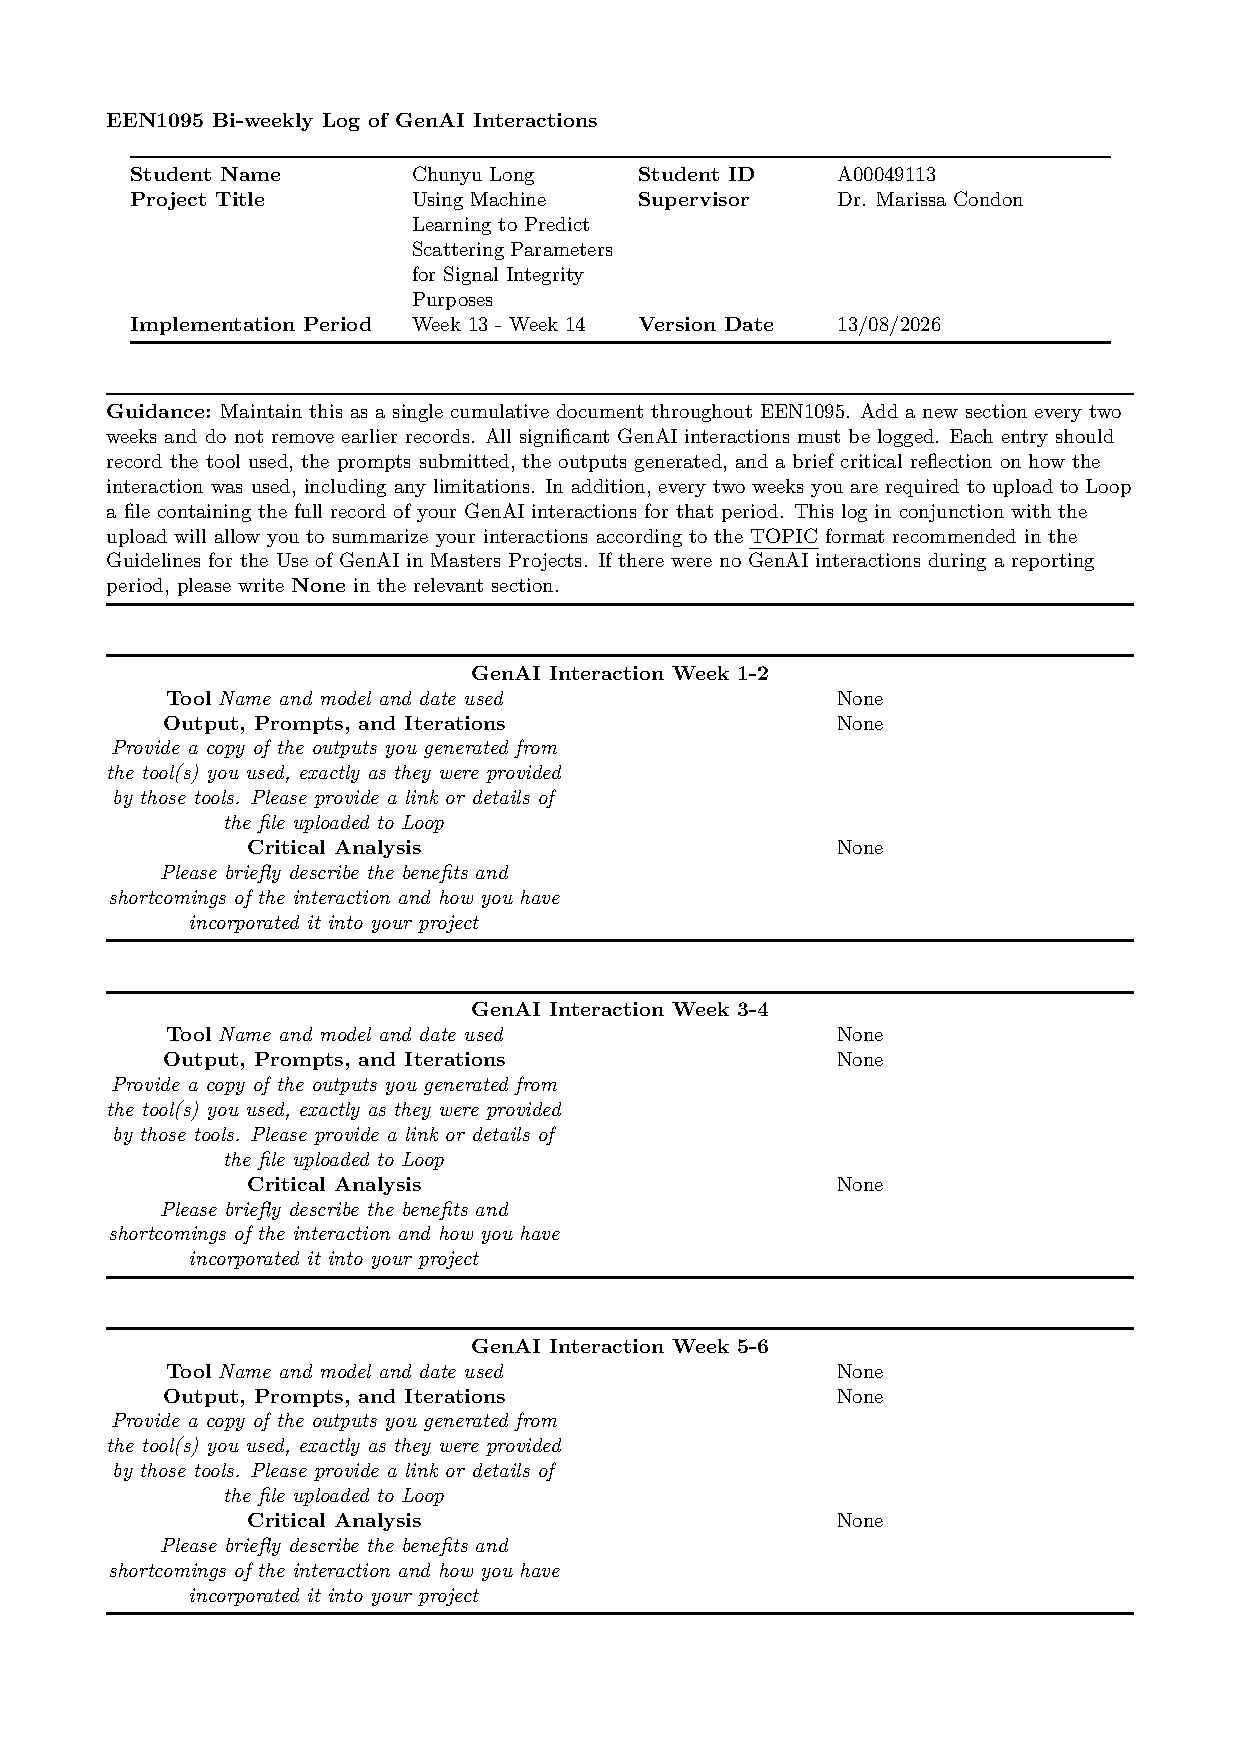
\includepdf[
    pages=-,
    fitpaper=true,
    pagecommand={\PortfolioImportedPageCommand},
    addtotoc={1,subsection,2,{A.2 Cumulative Bi-weekly GenAI Log},
              app:a-cumulative-log}
]{documents/EEN1095_Biweekly_GenAI_Log.pdf}


\PortfolioAppendixTitle{B}{Status Report}
\StartAppendixPages{B}
\addcontentsline{toc}{section}{Appendix B --- Status Report}
% !TEX root = ../main.tex
% Appendix B source fragment. Do not input this file into the six-page paper.
% The overall portfolio wrapper must load pdfpages, create the blank Appendix B
% title page, set B.1/B.2/... pagination and define the optional page hook below.
%
% The imported PDF is the unchanged EEN1101 submission. Do not edit, crop or
% regenerate it from the Word source.
\providecommand{\PortfolioImportedPageCommand}{}

\includepdf[
    pages=-,
    fitpaper=true,
    pagecommand={\PortfolioImportedPageCommand}
]{documents/ChunyuLong_A00049113_StatusReport.pdf}


\PortfolioAppendixTitle{C}{Project Plan, Progress, and Achievements}
\StartAppendixPages{C}
\addcontentsline{toc}{section}{Appendix C --- Project Plan, Progress, and
Achievements}
% Appendix C source fragment. Do not input this file into the six-page paper.
% The overall portfolio wrapper must load pdfpages and booktabs, create the
% blank Appendix C title page, establish C.1/C.2/... page numbering, and define
% the optional imported-page and content-page hooks below.
\providecommand{\PortfolioImportedPageCommand}{}
\providecommand{\PortfolioAppendixPageStyle}{}
\providecommand{\PortfolioContentPageCommand}{}

% C.1 is the complete approved plan. addtotoc records the subsection without
% placing new material over the original first page.

\includepdf[
    pages=-,
    fitpaper=true,
    pagecommand={\PortfolioImportedPageCommand},
    addtotoc={1,subsection,2,{C.1 Original Approved Plan},app:c-original-plan}
]{documents/ProjectPlan_A00049113_v4.0.pdf}

% The audit tables use the full page width for legibility. Return to two
% columns for the prose-based key-reference assessment in C.5.
\onecolumn
\PortfolioAppendixPageStyle
\PortfolioContentPageCommand
\phantomsection
\addcontentsline{toc}{subsection}{C.2 Progress and Key Milestones}
\subsection*{C.2 Progress and Key Milestones}
\label{app:c-progress}

The previous pages contain the complete approved EEN1101 project plan. The copy stored
in this portfolio is identical to the supplied PDF. Its SHA-256 digest is
\texttt{c6810b5da9e3a92a5a2417b596562a0d}\allowbreak
\texttt{c4d890c90e77b30b2d617e6ea173665e}.
Table~\ref{tab:appendix-c-progress} shows what was actually completed at each
planned stage. Dates in the selected run identifiers refer to the final saved
artifacts. They should not be read as a complete timeline of the exploratory
work.

In the evidence locations below, NB01 through NB08 identify the numbered
Jupyter notebooks in the submitted project repository. Appendix F maps each
label to its filename and purpose.

\begin{table}[!htbp]
    \caption{Progress and key milestones against the approved workplan.}
    \label{tab:appendix-c-progress}
    \centering
    \scriptsize
    \begin{tabular}{@{}p{0.16\textwidth}p{0.48\textwidth}
                         p{0.27\textwidth}@{}}
        \toprule
        Approved phase & What was completed & Evidence location \\
        \midrule
        Weeks 1--2:
        data pipeline
          & Linked 7,030 ten-parameter designs to complex 12-port Touchstone
            responses at 200 frequencies. All frequencies from a given design
            stayed in the same train, validation or test split. The resulting
            split contained 4,218/1,406/1,406 designs. Preprocessing was fitted
            on training data only.
          & Paper Section III; Appendix D, Shared Data and Leakage Controls;
            NB01 dataset analysis and NB02 preprocessing artifacts. \\
        Weeks 3--4:
        baselines
          & Built scalar and vector Ridge models, a powers-only Polynomial
            Ridge model and a Random Forest. Scalar Ridge achieved a test MAE
            of 7.5051~dB, compared with 12.3535~dB for the pooled global mean.
            However, it did not improve on the stronger 7.4254~dB
            frequency-dependent mean curve.
          & Paper Table I; Appendix E, Tables V--VII; NB03 selected runs. \\
        Weeks 3--6:
        point-wise neural exploration
          & Built two multilayer perceptrons with the common six-path interface.
            One used the original inputs. The other used a fifth-degree,
            powers-only expansion. Across the selected configurations, these
            models did not consistently reduce $IL_{7,1}$ error.
          & Paper Sections III--V; NB04 selected runs; Appendix D model
            descriptions and NB08 diagrams; Appendix E selected-run record. \\
        Weeks 5--7:
        whole-curve model
          & Built a model that maps one design to six curves at 200 frequencies.
            It uses a compact transposed-convolution decoder, fixed Fourier
            frequency coordinates and a curve-aware loss. The selected model
            achieved a test $IL_{7,1}$ MAE of 7.3883~dB.
          & Paper Sections III--V; Appendix D, Whole-Curve Neural Model;
            Appendix E paired comparisons; NB05 selected run. \\
        Weeks 6--9:
        complete matrix and diagnostics
          & Built a design-conditioned model for the reciprocal complex 12-port
            response. Its test complex MAE/NRMSE was 0.0686/0.7889. The
            training-mean matrix gave 0.0804/0.8343 on the same task.
            Reciprocity is exact by construction. Passivity and finite-band
            causality were checked after training.
          & Paper Sections III--V; Appendix D, Reciprocal Complete-Matrix
            Neural Model; Appendix E, Tables VIII--IX; NB06 selected run. \\
        Week 9:
        parameter study
          & The planned controlled sweep of every physical parameter was not
            completed. The final work therefore makes no parameter-sensitivity
            claim.
          & Paper limitations and future work; Tables
            \ref{tab:appendix-c-changes} and
            \ref{tab:appendix-c-objectives}. \\
        Final evaluation and
        portfolio
          & NB07 recomputed the selected metrics and produced the common-target
            and same-task comparisons. It also exported the physical
            diagnostics. The six-page paper was completed during the
            contingency period. NB08 and Appendices D--E provide the detailed
            implementation and testing record.
          & Paper; Appendices D--E; NB07--NB08; portfolio evidence exports. \\
        \bottomrule
    \end{tabular}
\end{table}

\clearpage
\PortfolioContentPageCommand
\phantomsection
\addcontentsline{toc}{subsection}{C.3 Major Changes to Scope or Methodology}
\subsection*{C.3 Major Changes to Scope or Methodology}
\label{app:c-changes}

Table~\ref{tab:appendix-c-changes} compares the approved method with the work
that was ultimately carried out. It also separates method changes from
objectives that were not completed. I use the label \emph{retrospective} when
no written approval or decision record was available from the time. I do not
describe a change as supervisor-approved unless written evidence confirms it.

\begin{table}[!htbp]
    \caption{Major method changes, reasons and consequences.}
    \label{tab:appendix-c-changes}
    \centering
    \scriptsize
    \begin{tabular}{@{}p{0.20\textwidth}p{0.27\textwidth}
                         p{0.25\textwidth}p{0.20\textwidth}@{}}
        \toprule
        Approved intent & What changed & Reason and evidence
                        & Consequence \\
        \midrule
        Row-wise input $[\mathbf u,f]$ with $2m^2$ real outputs at each
        design--frequency sample
          & The final model takes one design as input and generates the complete
            fixed 200-point response in one pass. It predicts 78 unique complex
            upper-triangle entries as 156 real channels.
          & \emph{Retrospective:} whole-grid prediction keeps the broadband
            context. Predicting only the upper triangle avoids learning
            reciprocal duplicates. The saved architecture and output contract
            confirm this change.
          & The complete-matrix objective was retained, but the approved
            formulation was not followed exactly. \\
        Complete matrix plus physical consistency
          & The predicted upper triangle is mirrored into the lower triangle.
          & The selected interconnect is passive and reciprocal. Reciprocity
            can therefore be built into the output structure, rather than
            learned twice from duplicate entries.
          & The prediction reciprocity residual is zero by construction. This
            structure does not enforce passivity or causality. \\
        Passivity and causality enforcement with a constrained/unconstrained
        comparison
          & Passivity and a finite-positive-band causality residual were checked
            after training. The selected loss gave zero weight to passivity and
            contained no causality term. A matched enforcement ablation was not
            completed.
          & \emph{Retrospective:} no passivity violation was found in the
            281,200 sampled test matrices. The selected model also did not show
            the non-physical negative insertion loss reported by Chen and Tan.
            With the time remaining, priority was given to complete-matrix
            prediction, diagnostics and a traceable evidence package.
          & Only reciprocity is guaranteed. Passivity is an observation on the
            sampled grid, while the finite-band causality result is a
            diagnostic. The planned enforcement and ablation remain unmet. \\
        Controlled variation of every physical parameter
          & The final controlled one-factor-at-a-time sweep was not completed.
          & \emph{Retrospective:} the remaining schedule was used to implement
            and validate the complete-matrix model. Completing the evidence
            package also took priority.
          & The effects on selected S-parameters, insertion loss, return loss
            and crosstalk were not established. \\
        Matrix MAE and RMSE as principal matrix errors
          & Complex MAE and complex NRMSE became the main matrix metrics. The
            common insertion-loss comparison still uses dB MAE and RMSE.
          & NRMSE relates the error to target energy. This is useful when matrix
            entries have different scales. Appendix E defines both metric
            domains.
          & The emphasis changed from RMSE to NRMSE for the complex matrix.
            Dimensionless complex errors remain separate from dB errors. \\
        Evaluation on unseen held-out data
          & Test designs were excluded from fitting. However, NB03--NB06
            inspected test results during development.
          & The progressive notebooks used test comparisons while the modelling
            path was still being developed.
          & The results are retrospective evidence on designs held out from
            fitting. They are not an untouched confirmatory test. \\
        Reduced repeated-simulation cost
          & Model inference time was recorded, but there was no matched timing
            measurement for electromagnetic simulation.
          & A comparable simulation run was not measured under a declared
            timing protocol.
          & The evidence does not support a simulation speed-up or cost-reduction
            claim. \\
        \bottomrule
    \end{tabular}
\end{table}

Several items remained intentionally outside the approved scope. These were
inverse design or geometry optimisation, a universal model spanning all
database topologies, production electronic-design-automation deployment, and
industrial replacement of electromagnetic simulation. They are not failed
objectives. The paper discusses cross-topology modelling only as future work.

\clearpage
\PortfolioContentPageCommand
\phantomsection
\addcontentsline{toc}{subsection}{C.4 Achievements Against Plan}
\subsection*{C.4 Achievements Against Plan}
\label{app:c-achievements}

Table~\ref{tab:appendix-c-objectives} gives one final status for each approved
objective or research-question component. ``Met with qualification'' means that
the core work was completed, but the evidence needs careful interpretation.
This applies when no acceptance threshold was set in advance or when a stronger
later check gives a more cautious result.

\begin{table}[!htbp]
    \caption{Approved objectives, final status and supporting evidence.}
    \label{tab:appendix-c-objectives}
    \centering
    \scriptsize
    \begin{tabular}{@{}p{0.24\textwidth}p{0.14\textwidth}
                         p{0.35\textwidth}p{0.18\textwidth}@{}}
        \toprule
        Approved objective or criterion & Status & Final evidence
                                         & Consequence \\
        \midrule
        Reproducible parameter/Touchstone pipeline by Week 2
          & Met, subject to final package audit
          & The pipeline contains 7,030 aligned designs. Split identifiers,
            training-only transforms, selected-run manifests and executable
            notebooks were saved.
          & I describe the workflow as ``documented and version-controlled''
            until Appendix F passes its clean-environment and accessibility
            audit. \\
        Baselines validate parsing, scaling, design splits and metrics by
        Week 3
          & Met with qualification
          & Scalar Ridge validation/test MAE was 7.3237/7.5051~dB. Its RMSE was
            10.8112/12.3342~dB. Test MAE improved on the 12.3535~dB pooled
            global mean, but not on the 7.4254~dB mean curve.
          & The baseline passes the specified global-mean comparison. The
            stronger frequency-dependent reference leads to a more cautious
            interpretation. \\
        Stable broadband neural prediction of the complete S-matrix by Week 6
          & Met with method change
          & Full-matrix test complex MAE/NRMSE was 0.0686/0.7889, compared with
            0.0804/0.8343 for the same-task mean matrix. Representative
            reflection and crosstalk responses were retained.
          & The approved row-wise implementation was replaced by a reciprocal
            design-to-grid formulation. \\
        Reproduce main broadband trends on held-out designs
          & Partly met
          & Aggregate errors and representative complex curves show that the
            main trends were reproduced for sampled designs. Confidence is
            limited by one selected seed and development-time test exposure.
          & The test evidence is not untouched. It also does not establish
            universal generalisation. \\
        Enforce passivity and causality and compare constrained/unconstrained
        variants by Week 8
          & Unmet
          & The reciprocity residual was 0. There were 0 passivity violations
            in 281,200 predicted matrices, and the maximum singular value was
            0.9141. The test prediction/truth finite-band causality residual was
            0.4812/0.3173. No enforcement ablation was completed.
          & These results are diagnostics. Passivity on the sampled test grid
            is not a global guarantee. \\
        Vary every physical parameter with others controlled by Week 9
          & Unmet
          & No final one-factor-at-a-time study was produced. The planned
            insertion-loss, return-loss and crosstalk analysis is also absent.
          & This remains evidence-led future work. No sensitivity claim is
            made. \\
        Final comparison with relevant broadband methods
          & Partly met
          & Paper Sections II and V compare target scope, broadband interface,
            complex representation and physical mechanisms with the five key
            works assessed in C.5.
          & The comparison remains qualitative where datasets or metrics
            differ. Missing enforcement and parameter evidence are stated
            directly. \\
        Accuracy sufficient for signal-integrity decisions
          & Not established
          & Numerical error was quantified. However, no downstream decision,
            engineering tolerance or acceptance threshold was defined.
          & The evidence does not establish task-level sufficiency or industrial
            usefulness. \\
        Reduce repeated electromagnetic-simulation cost
          & Not established
          & No matched simulation timing baseline was collected.
          & Inference timing alone cannot support a simulation speed-up claim. \\
        \bottomrule
    \end{tabular}
\end{table}

Overall, the approved composite research question was only partly answered.
The project produced a design-conditioned approximation of the complete
reciprocal complex response for one topology. It also quantified prediction
error and physical behaviour on the sampled test grid. The work did not
establish task-specific signal-integrity sufficiency. It also did not complete
passivity or causality enforcement, the controlled parameter study, or a
comparison of cost with electromagnetic simulation.

\twocolumn
\PortfolioAppendixPageStyle
\PortfolioContentPageCommand
\phantomsection
\addcontentsline{toc}{subsection}{C.5 Key References for Detailed Assessment}
\subsection*{C.5 Key References for Detailed Assessment}
\label{app:c-key-references}

These five sources provide the main foundation for the dataset, broadband
representation, physical-validity motivation, complex prediction and multi-port
comparison. Their bracketed numbers match the current six-page paper. If the
paper's bibliography order changes, these labels must be updated before
submission.

\subsubsection*{Paper reference [1] --- Schierholz et al.}
M. Schierholz, A. S\'{a}nchez-Mas\'{i}s, A. Carmona-Cruz, X. Duan, K. Roy,
C. Yang, R. Rimolo-Donadio, and C. Schuster, ``SI/PI-Database of PCB-Based
Interconnects for Machine Learning Applications,'' \emph{IEEE Access}, vol. 9,
pp. 34423--34432, 2021, doi: 10.1109/ACCESS.2021.3061788.

Schierholz \textit{et al.} introduce the open PCB-interconnect database used in
this project. They also demonstrate neural prediction of selected S-parameter
magnitude and phase. A key strength is the public pairing of parameterised
geometries with simulated Touchstone responses. The authors report lower
accuracy for electrically longer, more frequency-dependent links. This finding
is directly relevant to the selected topology. Their study focuses on selected
responses rather than a design-conditioned complete complex 12-port matrix.
This project uses one of their datasets and keeps designs separate across the
data splits. It extends prediction to the complete matrix, but remains limited
to one topology.

\subsubsection*{Paper reference [3] --- Torun et al.}
H. M. Torun, H. Yu, N. Dasari, V. C. K. Chekuri, A. Singh, J. Kim, S. K. Lim,
S. Mukhopadhyay, and M. Swaminathan, ``A Spectral Convolutional Net for
Co-Optimization of Integrated Voltage Regulators and Embedded Inductors,'' in
\emph{Proc. IEEE/ACM Int. Conf. Computer-Aided Design}, 2019, pp. 1--8,
doi: 10.1109/ICCAD45719.2019.8942109.

Torun \textit{et al.} propose a spectral transposed-convolutional network. It
generates an entire frequency response instead of treating each frequency
independently. The architecture uses local spectral structure and is well
suited to broadband outputs. However, its application and targets differ from
the 12-port PCB problem. It also does not guarantee passivity or causality. This
project adapts the transposed-convolution idea to six insertion-loss curves. It
adds fixed frequency coordinates and a curve-aware loss. The resulting model is
described as S-TCNN-style, not as an exact reproduction.

\subsubsection*{Paper reference [4] --- Chen and Tan}
L. Chen and L. Tan, ``Physics-Enforced Modeling for Insertion Loss of
Transmission Lines by Deep Neural Networks,'' in \emph{Proc. 2021 IEEE
Asia-Pacific Microwave Conf.}, 2021, pp. 276--278,
doi: 10.1109/APMC52720.2021.9661782.

Chen and Tan show that an unconstrained neural model can produce non-physical
negative insertion loss. They add physical enforcement to address this
behaviour. Their study clearly shows why numerical error alone is not enough
for a signal-integrity surrogate. However, it considers a selected insertion-
loss response rather than a complete complex multi-port matrix. In this
project, their result motivates the physical diagnostics. The selected
full-matrix predictions did not show the reported behaviour on the sampled test
grid, but the enforcement experiment was not reproduced.

\subsubsection*{Paper reference [5] --- Akinwande et al.}
O. Akinwande, S. Erdogan, R. Kumar, and M. Swaminathan, ``Surrogate Modeling
With Complex-Valued Neural Nets for Signal Integrity Applications,''
\emph{IEEE Trans. Microwave Theory Tech.}, vol. 72, no. 1, pp. 478--489,
Jan. 2024, doi: 10.1109/TMTT.2023.3319835.

Akinwande \textit{et al.} predict broadband complex $S_{11}$ and $S_{21}$ with
a complex-valued network. Their work combines phase-bearing responses with
passivity and causality considerations. However, the evaluated output is a
selected subset rather than every entry in a high-port-count matrix. This
project also preserves real and imaginary information. It uses paired
real-valued channels and predicts the complete reciprocal matrix. Only
reciprocity is enforced; passivity and causality remain diagnostics.

\subsubsection*{Paper reference [6] --- Karahan et al.}
E. A. Karahan, Z. Liu, A. Gupta, Z. Shao, J. Zhou, U. Khankhoje, and
K. Sengupta, ``Deep-Learning Enabled Generalized Inverse Design of Multi-Port
Radio-Frequency and Sub-Terahertz Passives and Integrated Circuits,''
\emph{Nature Communications}, vol. 15, art. 10734, 2024,
doi: 10.1038/s41467-024-54178-1.

Karahan \textit{et al.} demonstrate deep-learning models for complex multi-port
responses and inverse design across radio-frequency and sub-terahertz
structures. Their broad multi-port scope is important because it shows that
complex multi-port learning is not new by itself. However, their structures,
datasets, inverse-design aim and evaluation protocol differ from this PCB
interconnect problem. The present project has a narrower aim. It is a
forward-only, topology-specific study of the complete reciprocal broadband
12-port response. For this reason, no cross-paper numerical ranking is made.


\PortfolioAppendixTitle{D}{Design and Implementation Details}
\StartAppendixPages{D}
\twocolumn
\appendices
\setcounter{section}{3}
% Appendix D source fragment. Do not input this file into the six-page paper.
% The overall portfolio wrapper should provide the Appendix D title page and
% appendix numbering before inputting this content.
\section{Design and Implementation Details}
\label{app:design-implementation}

\subsection{Purpose and Design Progression}
This appendix records the implementation detail omitted from the six-page
paper. The project progressed through four modelling questions:

\begin{enumerate}
    \item Can simple point-wise models establish a credible reference?
    \item Does generic nonlinearity improve the selected insertion-loss paths?
    \item Does predicting complete broadband curves jointly provide a better
          representation of frequency structure?
    \item Can one model predict the reciprocal complete complex 12-port
          scattering matrix over the fixed frequency grid?
\end{enumerate}

The sequence is an exploration path, not a claim that each later model is more
accurate. The notation $IL_{7,1}$ denotes insertion loss from input port 1 to
output port 7. Table~\ref{tab:appendix-d-interfaces} shows that the later stages
also change the output scope and data interface. Consequently, comparisons are
used to reveal trade-offs rather than to attribute every difference to one
isolated architectural choice.

\begin{table*}[t]
    \caption{Implemented model interfaces. The batch dimension is omitted.}
    \label{tab:appendix-d-interfaces}
    \centering
    \scriptsize
    \begin{tabular}{@{}llll@{}}
        \toprule
        Stage & Model input & Model output & Main question \\
        \midrule
        Point-wise scalar
          & 10 design values + frequency
          & one $IL_{7,1}$ value
          & basic linear reference \\
        Point-wise vector
          & 10 design values + frequency
          & six insertion-loss values
          & output packaging and nonlinearity \\
        Whole curve
          & 10 design values + fixed frequency features
          & $200\times6$ insertion-loss tensor
          & joint broadband representation \\
        Full matrix
          & 10 design values; internal fixed frequency features
          & $200\times156$ unique real-valued channels
          & complete reciprocal complex response \\
        \bottomrule
    \end{tabular}
\end{table*}

\subsection{Shared Data and Leakage Controls}
All stages used the same 7,030 aligned designs and the project seed 128. The
design-level split contained 4,218 training, 1,406 validation and 1,406 test
designs. Every frequency belonging to one design stayed in the same split.
Training data fitted model parameters and all scaling or feature transforms;
validation data selected configured alternatives and neural checkpoints. Test
designs were excluded from fitting, although their results were inspected
during development, so the final evaluation is retrospective rather than an
untouched confirmation.

The point-wise table contains one row per design and frequency. Its 11 inputs
are ten physical design parameters plus frequency in gigahertz (GHz). The curve
and matrix models retain one sample per design and generate all 200 frequencies
together. This change avoids treating each frequency row as a separate training
sample, but it also means that a point-wise/curve comparison changes more than
the network architecture.

Each model owns its preprocessing so that saved predictions can be reproduced:

\begin{itemize}
    \item Ridge and point-wise neural models standardise their inputs using
          training data. Their insertion-loss targets are also standardised for
          neural training.
    \item Polynomial models expand each input independently and then fit a
          second training-only standardisation. No cross-feature interaction
          terms are generated by this powers-only expansion.
    \item Random Forest uses the original unscaled inputs because tree splits
          depend on ordering rather than feature magnitude.
    \item The whole-curve model standardises the ten design inputs and each of
          its six target channels using pooled training-curve values.
    \item The full-matrix model standardises the design inputs. Each complex
          matrix entry uses one training-set root-mean-square scale shared by
          its real and imaginary parts, preserving their relative scale.
\end{itemize}

\subsection{Non-Neural Point-Wise Models}
\subsubsection{Ridge Regression}
Ridge regression fits a linear mapping while discouraging very large
coefficients. For input matrix $\mathbf X$, target matrix $\mathbf Y$ and
coefficient matrix $\mathbf W$, the fitted objective is
\begin{equation}
    \min_{\mathbf W}
    \left\|\mathbf Y-\mathbf X\mathbf W\right\|_F^2
    +\alpha\left\|\mathbf W\right\|_F^2.
    \label{eq:appendix-d-ridge}
\end{equation}
The scalar version predicts only $IL_{7,1}$. The vector version predicts six
corresponding left-to-right insertion-loss paths. Multi-output Ridge fits one
coefficient vector per target; it does not create a learned coupling between
the outputs. The common selected regularisation value was $\alpha=0.01$.

The scalar model established whether design and frequency features could beat
a pooled training mean. The vector model then established a common six-output
interface for the nonlinear point-wise models. Their identical $IL_{7,1}$
solution is therefore expected and is not evidence that adding outputs improves
the scalar target.

\subsubsection{Polynomial Ridge}
Polynomial Ridge tests explicit smooth nonlinearity without changing the
linear estimator. Each standardised input $x_j$ is expanded independently as
\begin{equation}
    x_j\mapsto[x_j,x_j^2,\ldots,x_j^D].
    \label{eq:appendix-d-polynomial-map}
\end{equation}
Validation selected degree $D=3$ and $\alpha=50$. The expansion contains no
terms such as $x_jx_k$, which keeps the model compact but prevents it from
representing interactions explicitly. This was an intentional intermediate
step between linear Ridge and more flexible learned or tree-based mappings.

\subsubsection{Random Forest}
Random Forest averages 128 regression trees. Each tree recursively divides the
joint design--frequency space into regions and predicts the mean target within
each terminal region. Bootstrap samples diversify the trees before averaging;
the selected implementation makes every input feature available at each split.
Validation retained a minimum of two samples per leaf and unrestricted maximum
depth. The model can represent local interactions without polynomial feature
engineering, but its piecewise predictions do not encode smoothness along
frequency.

\begin{table*}[t]
    \caption{Selected non-neural configurations and their design roles.}
    \label{tab:appendix-d-non-neural}
    \centering
    \scriptsize
    \begin{tabular}{@{}lllll@{}}
        \toprule
        Model & Outputs & Transform & Selected setting & Design role \\
        \midrule
        Scalar Ridge
          & 1 & standardisation & $\alpha=0.01$
          & weak linear baseline \\
        Vector Ridge
          & 6 & standardisation & $\alpha=0.01$
          & common six-output baseline \\
        Polynomial Ridge
          & 6 & powers + standardisation & degree 3, $\alpha=50$
          & explicit smooth nonlinearity \\
        Random Forest
          & 6 & none & 128 trees, leaf $\geq2$
          & local nonlinear interactions \\
        \bottomrule
    \end{tabular}
\end{table*}

These scikit-learn estimators do not have Keras computation graphs. Equations,
the transformation description and Table~\ref{tab:appendix-d-non-neural} are
therefore more informative than forcing them into neural-network-style layer
diagrams.

\subsection{Point-Wise Neural Models}
A multilayer perceptron (MLP) is a feed-forward neural network in which every
unit in one layer connects to every unit in the next. The raw-input MLP accepts
the 11 standardised design--frequency features. Three hidden layers contain
128, 128 and 64 units with rectified linear unit (ReLU) activation, followed by
a linear six-unit output. It has 26,694 trainable parameters.

The Polynomial Neural MLP uses the same hidden and output layers after a fixed
fifth-degree powers-only expansion. Eleven original inputs therefore become 55
expanded inputs before the training-fitted standardisation, increasing the
network to 32,326 parameters. Comparing the two MLPs tests the value of explicit
univariate powers while keeping the learned hidden architecture fixed.

\begin{figure*}[p]
    \centering
    \begin{minipage}[t]{0.46\textwidth}
        \centering
        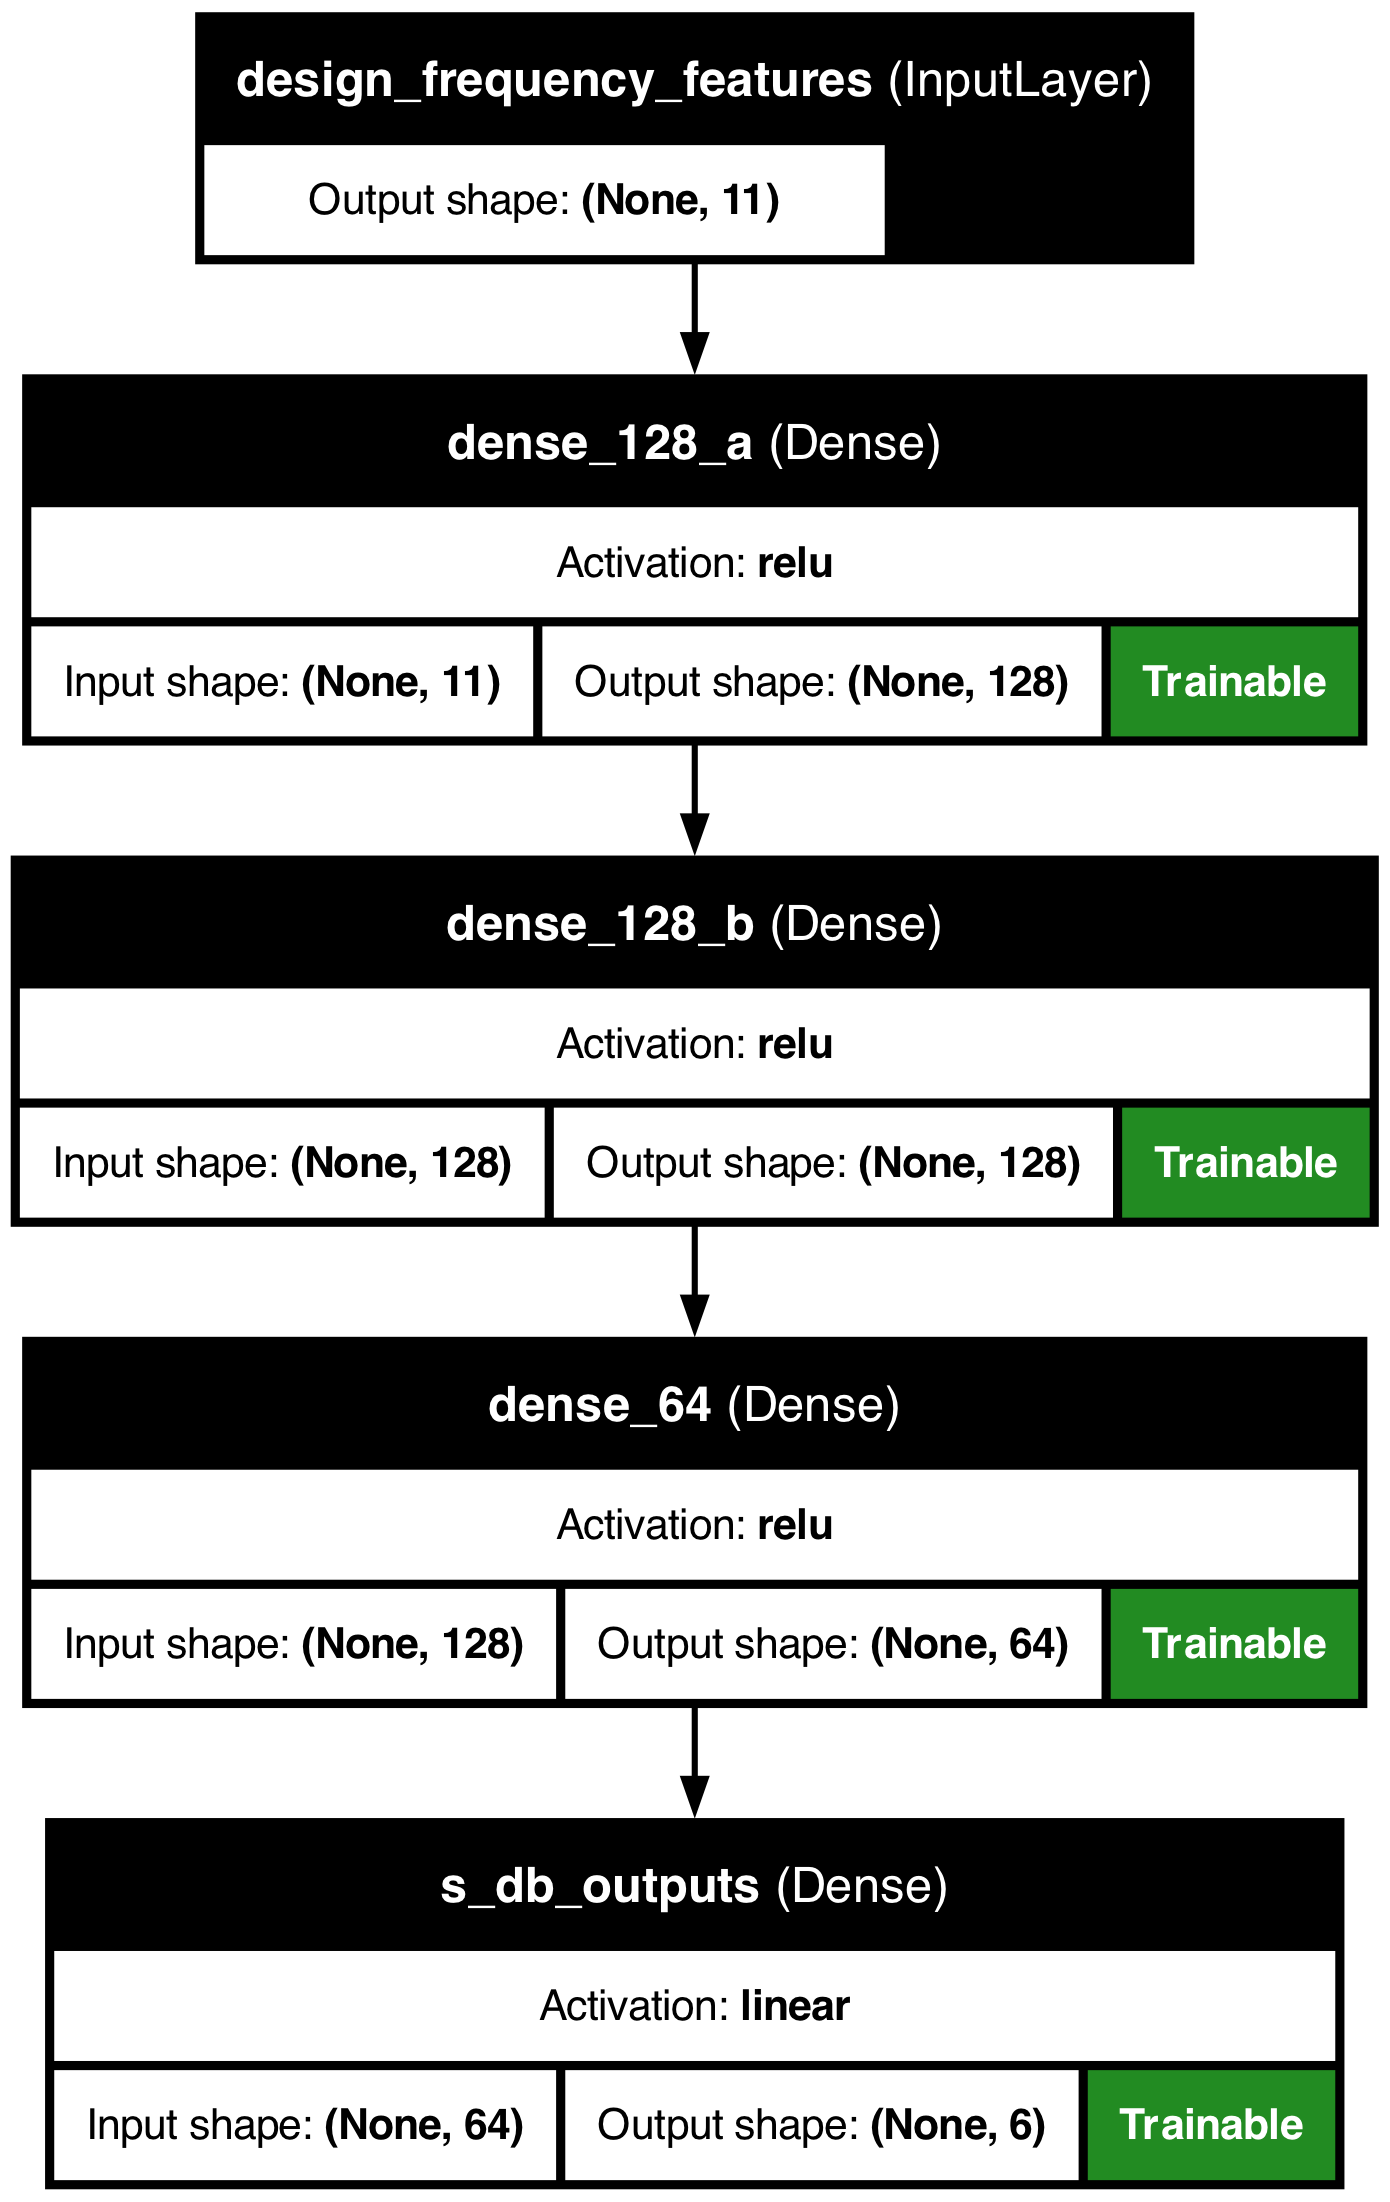
\includegraphics[width=\linewidth,height=0.72\textheight,
                         keepaspectratio]
          {appendix_d/neural_mlp_topology.png}
    \end{minipage}\hfill
    \begin{minipage}[t]{0.46\textwidth}
        \centering
        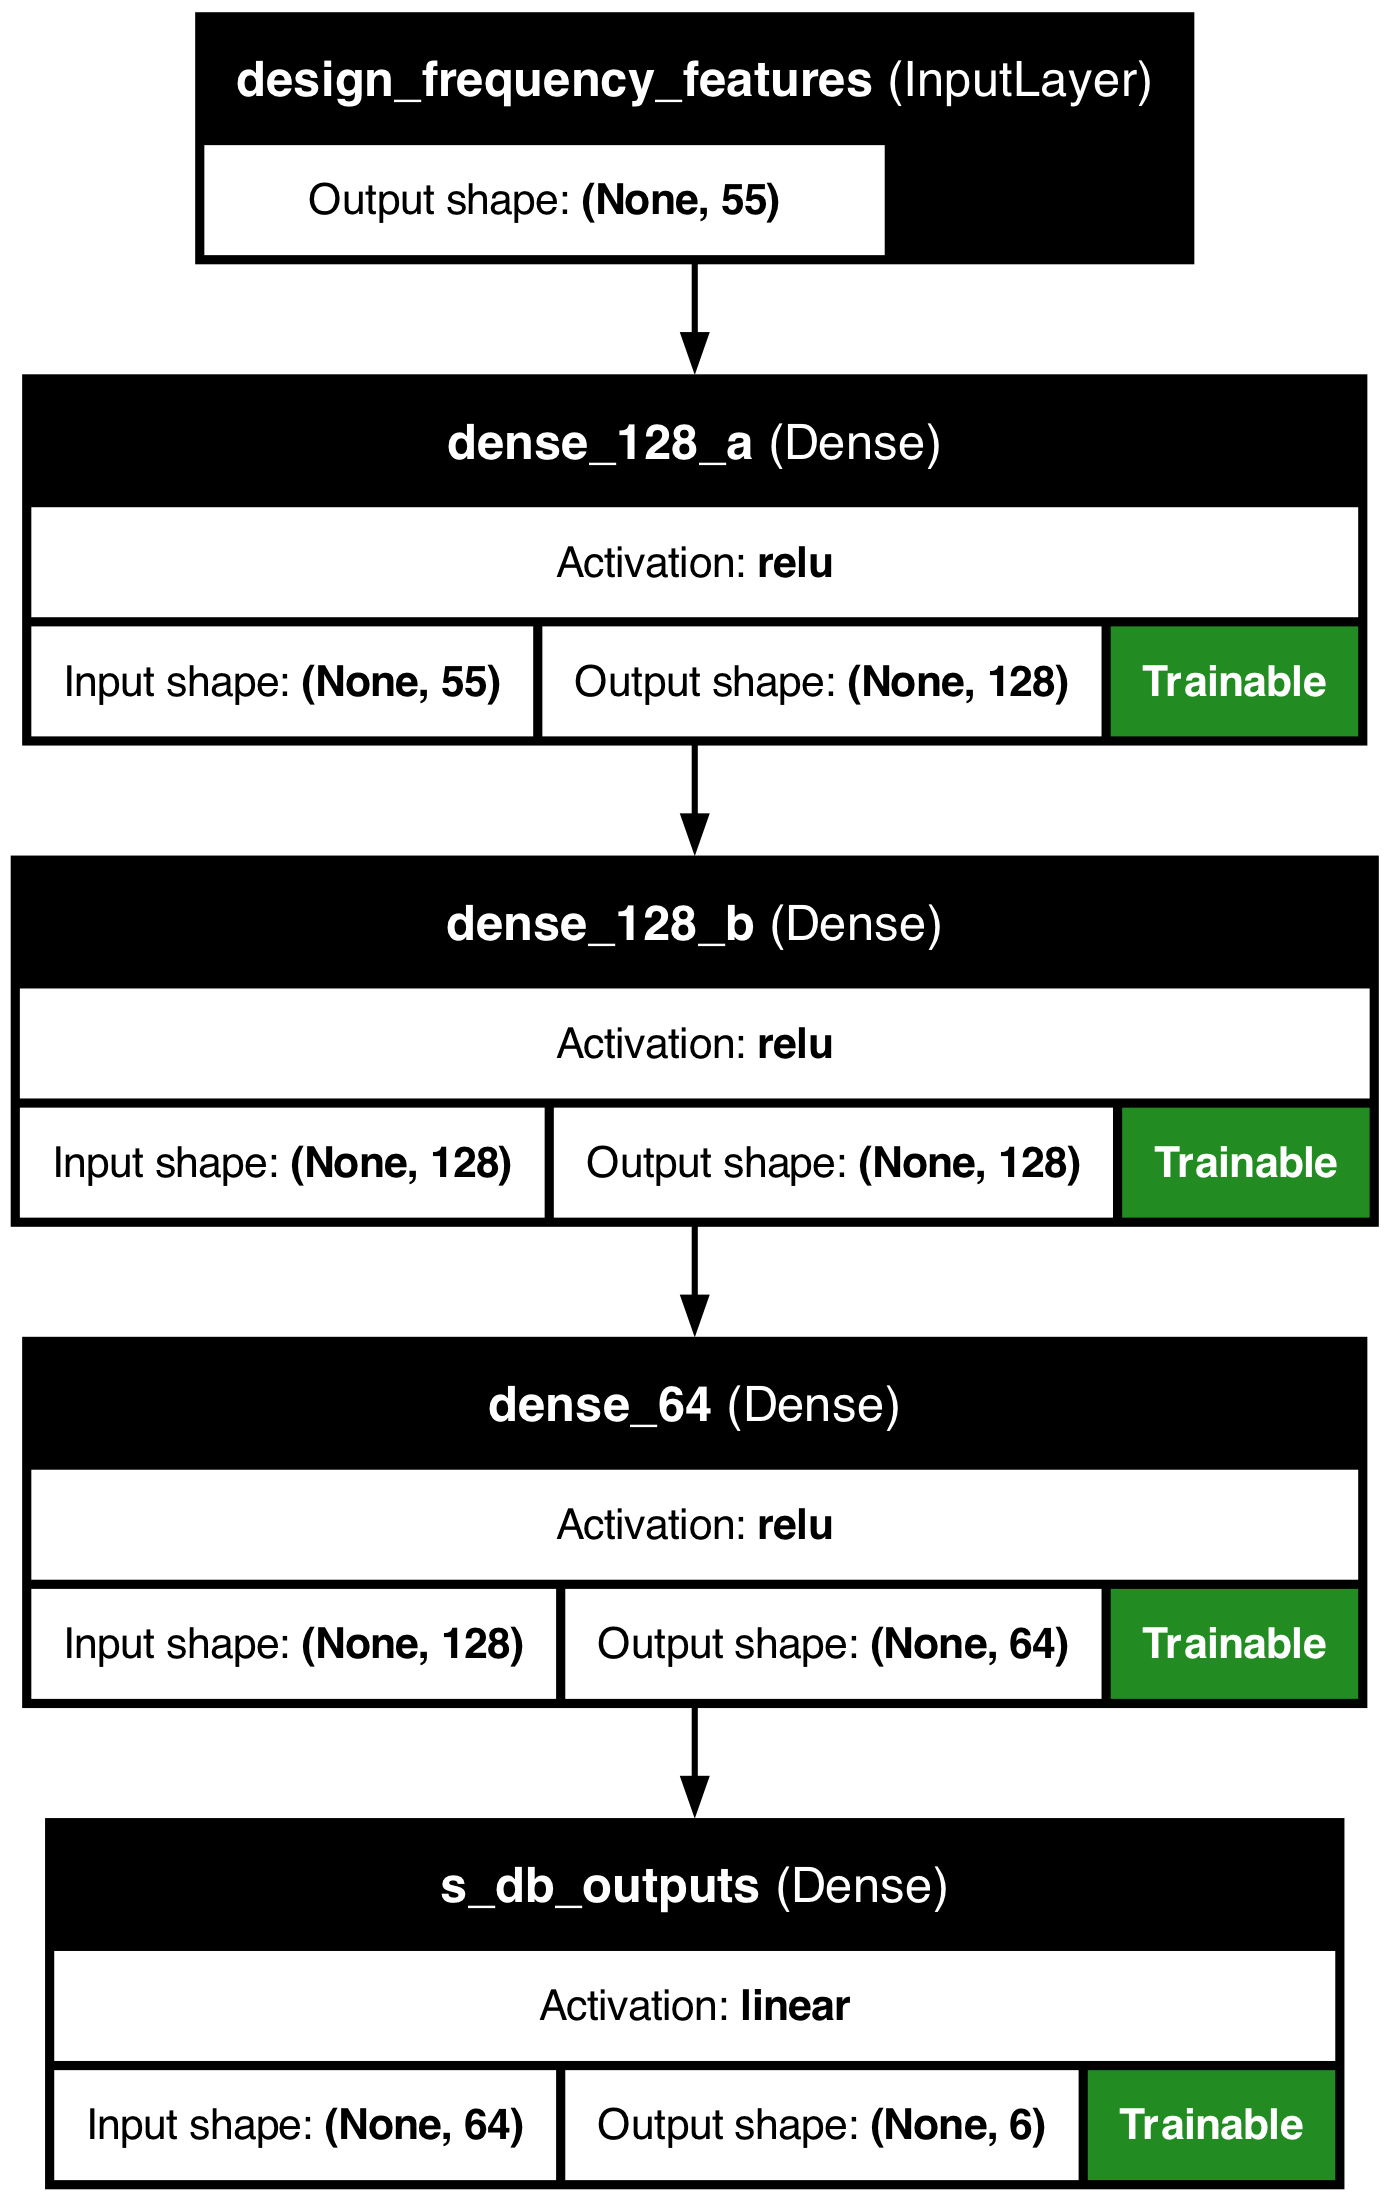
\includegraphics[width=\linewidth,height=0.72\textheight,
                         keepaspectratio]
          {appendix_d/polynomial_neural_mlp_topology.png}
    \end{minipage}
    \caption{Saved point-wise MLP topologies. The raw-input model is shown on
    the left and the polynomial-input model on the right. The graphs are
    generated from the selected Keras artifacts; preprocessing occurs outside
    the displayed networks. ``None'' denotes the variable batch dimension.}
    \label{fig:appendix-d-pointwise-mlp}
\end{figure*}

Both networks minimise mean squared error (MSE) in standardised target space
using the Adam optimiser. Training uses batches of 512, an initial learning rate
of $3\times10^{-5}$ and gradient-norm clipping at 0.5. A validation-loss plateau
reduces the learning rate; early stopping restores the best validation
checkpoint. The maximum of 100 epochs is a ceiling rather than a requirement to
retain the last epoch.

\subsection{Whole-Curve Neural Model}
The whole-curve model accepts one ten-parameter design and returns six complete
200-point insertion-loss curves. It is inspired by a spectral transposed
convolutional neural network (S-TCNN), but is not an exact reproduction of the
published architecture. The selected implementation contains 35,870 trainable
parameters and proceeds as follows:

\begin{enumerate}
    \item A 32-unit dense encoder maps the design vector to a latent state.
    \item A dense projection creates 800 values and reshapes them to 25
          positions with 32 channels.
    \item Three one-dimensional transposed convolutions double the sequence
          length from 25 to 50, 100 and 200 positions, with 32, 16 and 8
          channels respectively.
    \item Nine fixed frequency coordinates---normalised frequency plus four
          sine/cosine pairs---are concatenated at each output position.
    \item A one-dimensional refinement convolution and a linear six-channel
          convolution return the $200\times6$ insertion-loss tensor.
\end{enumerate}

\begin{figure*}[p]
    \centering
    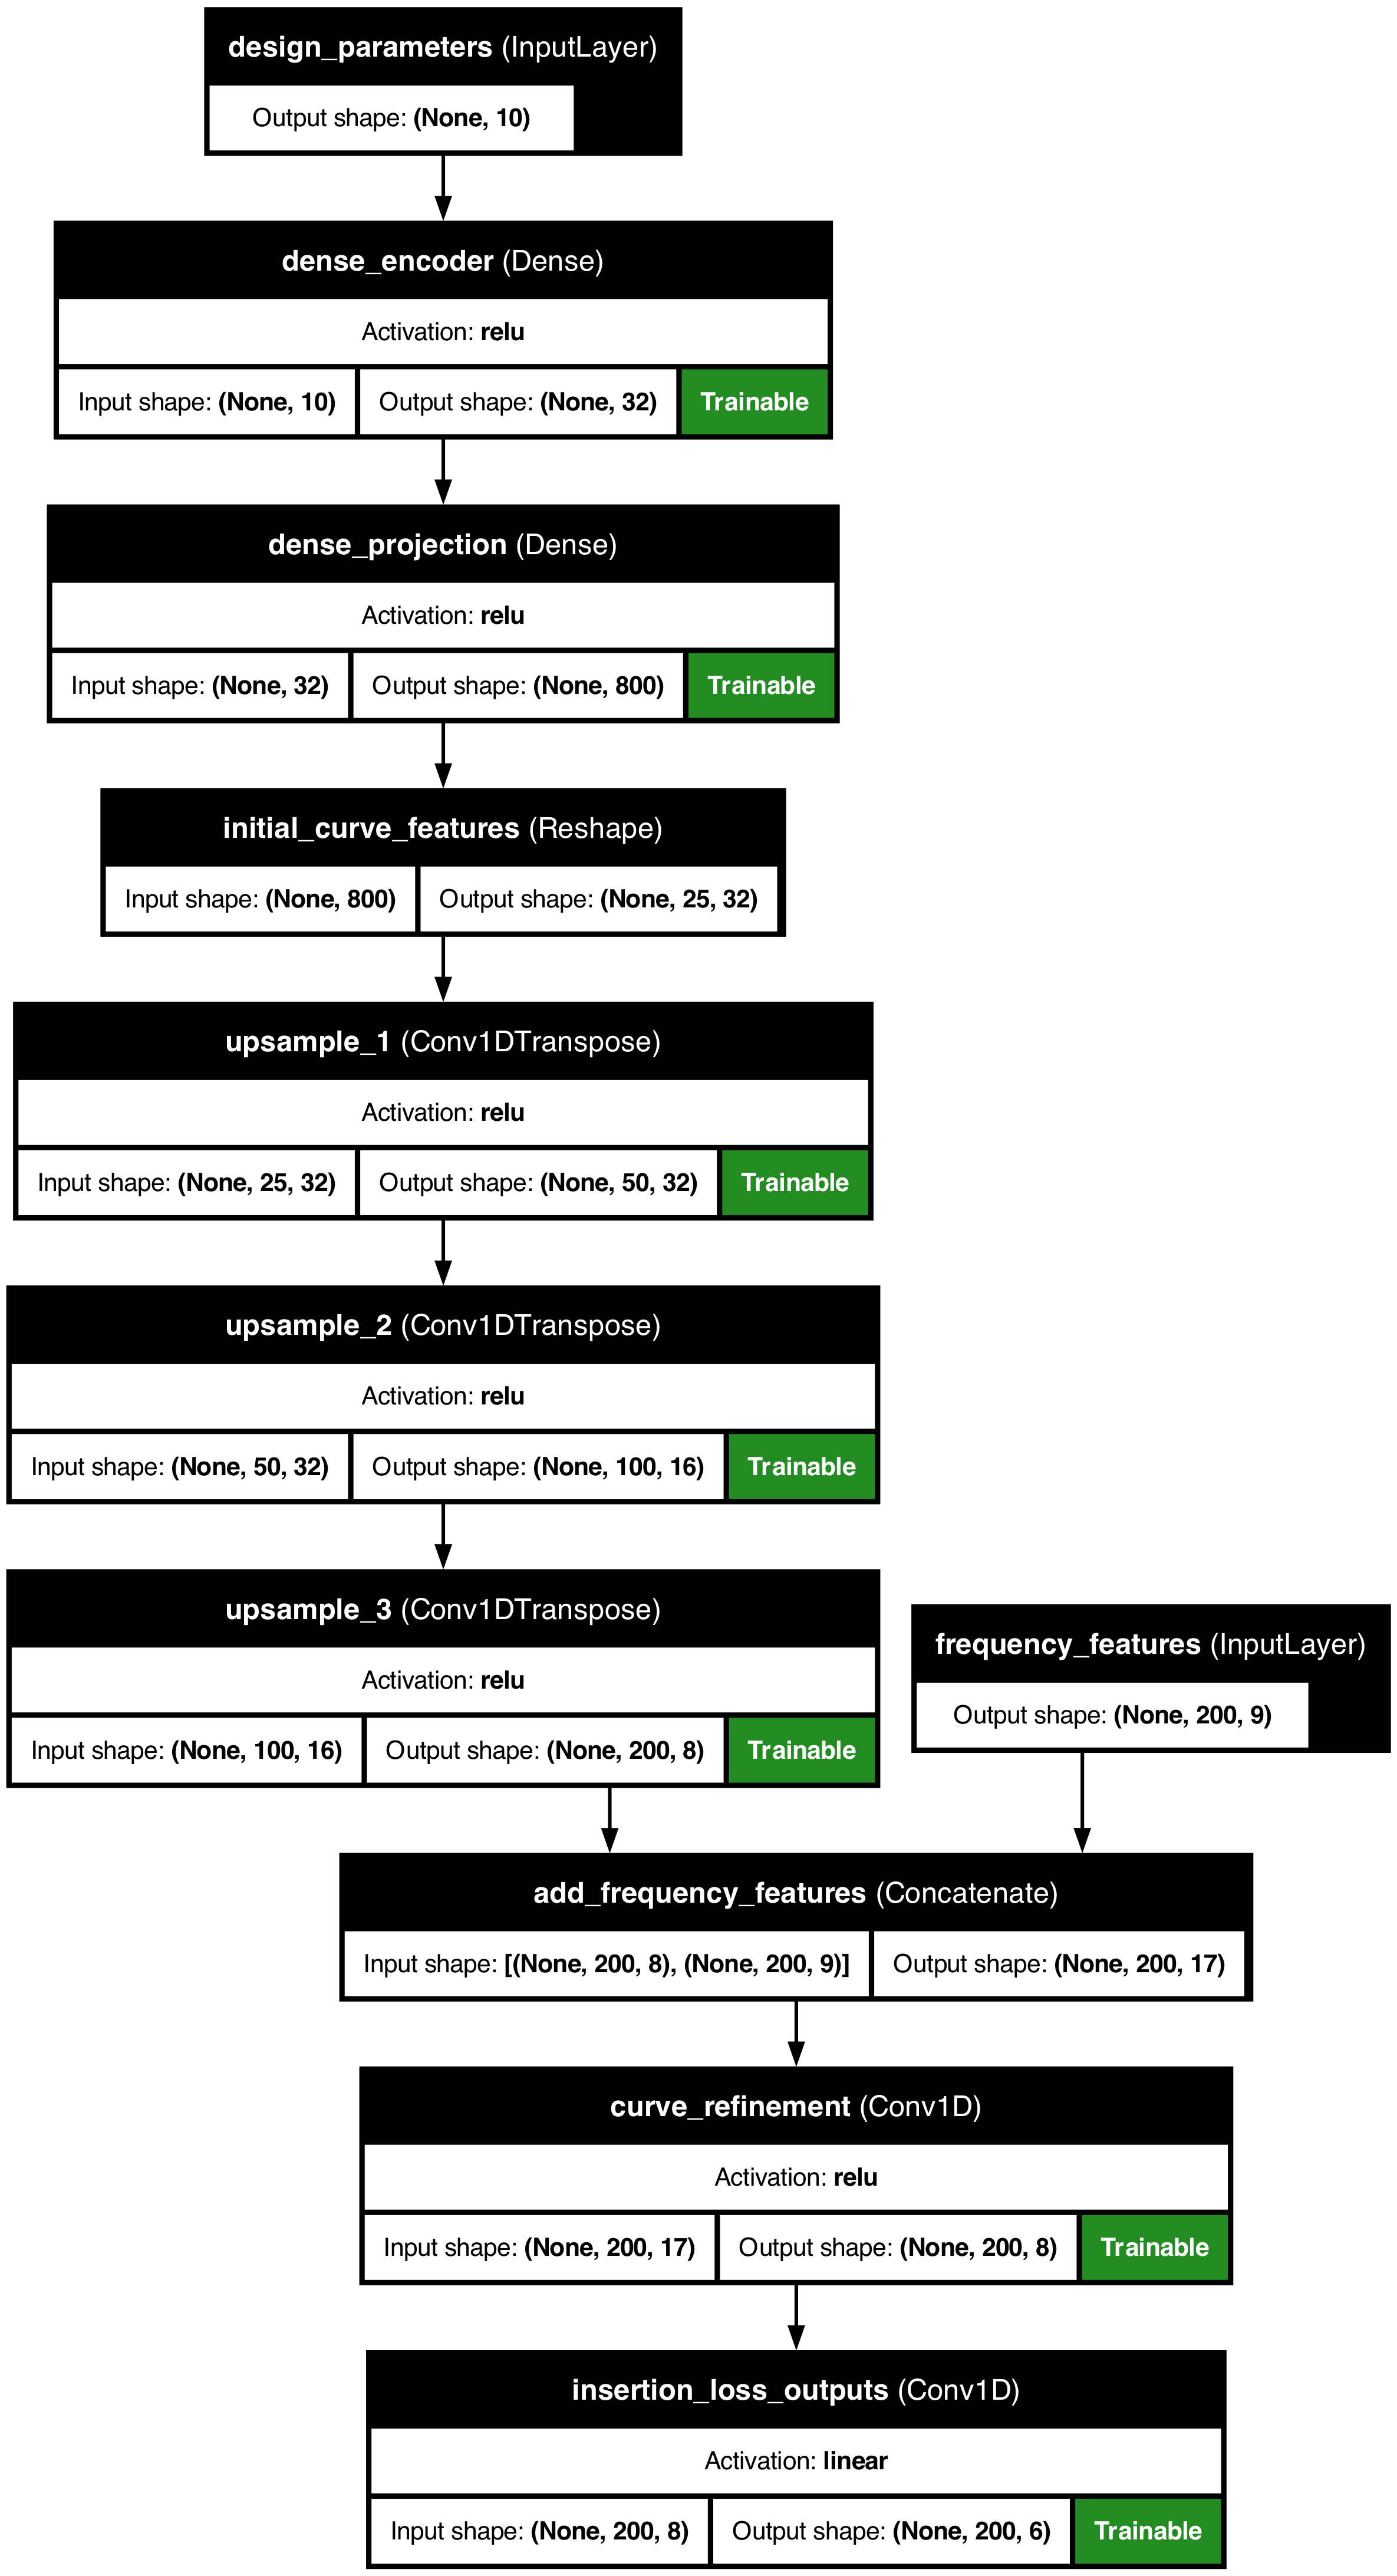
\includegraphics[height=0.87\textheight,keepaspectratio]
      {appendix_d/curve_neural_topology.png}
    \caption{Topology of the selected whole-curve neural model. Transposed
    convolutions expand the latent sequence to 200 frequencies before the fixed
    frequency coordinates and final curve-refinement layers are applied.}
    \label{fig:appendix-d-curve-topology}
\end{figure*}

The selected curve loss combines point-wise MSE with error in the first
difference along frequency:
\begin{equation}
    \mathcal L_{\mathrm{curve}}
      =\operatorname{MSE}(\widehat{\mathbf L},\mathbf L)
      +\lambda_{\Delta}\operatorname{MSE}
       (\Delta_f\widehat{\mathbf L},\Delta_f\mathbf L).
    \label{eq:appendix-d-curve-loss}
\end{equation}
The training-derived weight $\lambda_{\Delta}=11.626038$ makes the derivative
term contribute 10\% of the point-wise MSE on the training reference. Validation
experiments compared absent, linear and Fourier frequency coordinates;
current-size and compact decoders; and point-wise and curve-aware losses. The
compact Fourier, curve-aware configuration was retained. Because interface,
scaling, architecture and loss changed together, its comparison with the
point-wise MLP is not a controlled ablation of frequency structure alone.

Training uses Adam with an initial learning rate of $10^{-3}$, batches of 64,
gradient clipping at 0.5 and a maximum of 100 epochs. Learning-rate reduction
and early stopping monitor inverse-scaled validation mean absolute error (MAE)
across all six curves.

\subsection{Reciprocal Complete-Matrix Neural Model}
The final model maps one design to the complete complex response at 200
frequencies. Its external data contract contains real and imaginary parts for
all $12^2=144$ entries, or 288 real values per frequency. Internally, it predicts
only the 78 unique upper-triangle complex entries, represented by 156 real
channels, and constructs the remaining entries by
\begin{equation}
    \widehat S_{i,j}(f_k)=\widehat S_{j,i}(f_k),\qquad i>j.
    \label{eq:appendix-d-reciprocity}
\end{equation}
This guarantees reciprocity exactly while avoiding duplicate learned outputs.
It does not enforce passivity or causality.

The network has 125,852 trainable parameters. The ten standardised design values
are repeated over the 200-point grid. At each frequency they are concatenated
with 41 fixed coordinates: normalised frequency, four Fourier sine/cosine pairs
and 32 Gaussian radial-basis features. A dense projection produces 128 features.
Three width-128 residual blocks then learn corrections while skip connections
preserve a direct route through each block. A final linear layer produces the
$200\times156$ scaled real/imaginary output.

\begin{figure*}[p]
    \centering
    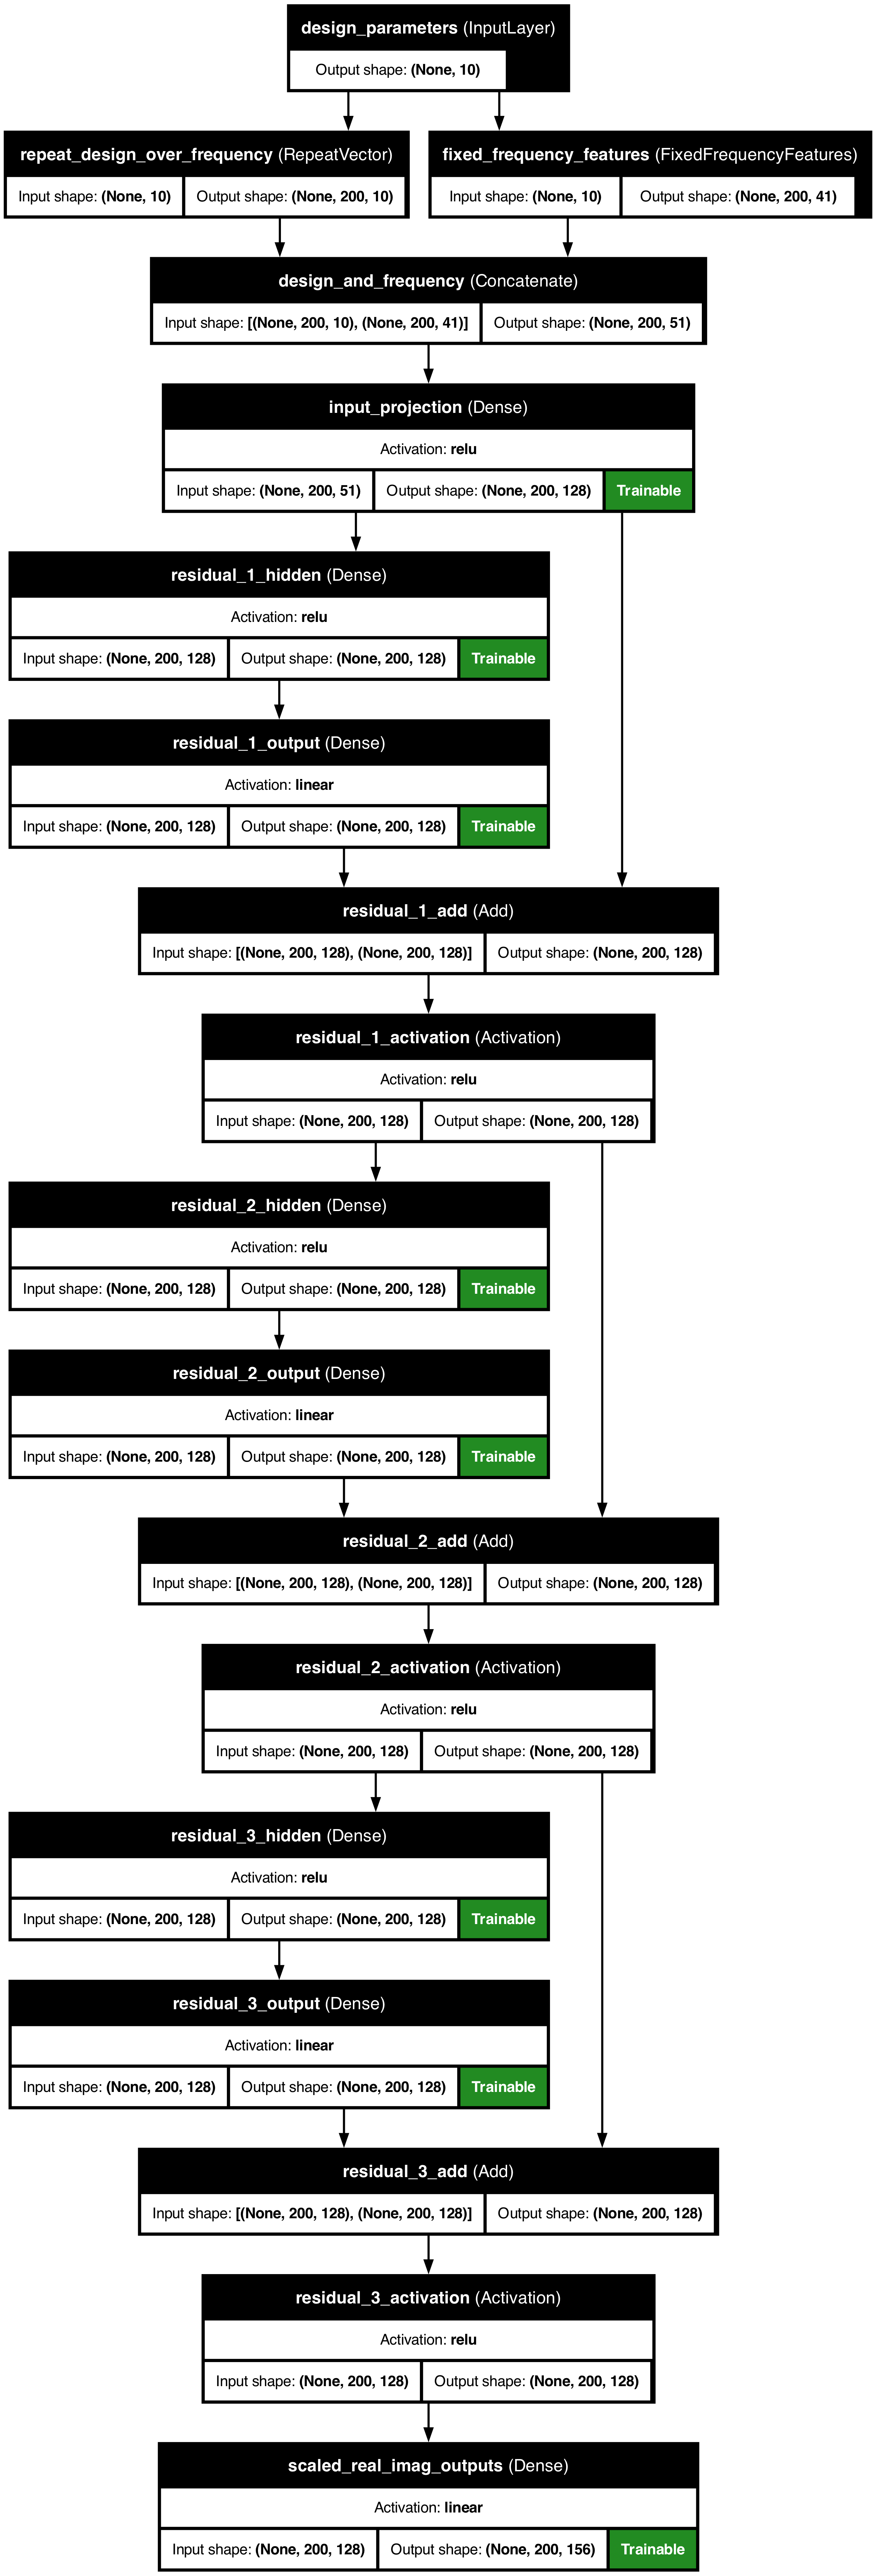
\includegraphics[height=0.90\textheight,keepaspectratio]
      {appendix_d/full_smatrix_neural_topology.png}
    \caption{Topology of the selected frequency-conditioned full-matrix neural
    model. The graph ends at the 156 unique real-valued channels. Reciprocal
    mirroring and inverse scaling occur in the model wrapper after this Keras
    graph.}
    \label{fig:appendix-d-full-matrix-topology}
\end{figure*}

The selected loss combines normalised complex MSE with a weight-0.1 Huber loss
on off-diagonal log magnitude. The log-magnitude term reduces the dominance of
large responses and gives weak transmission/crosstalk entries a direct training
signal. The passivity weight is zero and there is no causality loss. Validation
complex normalised root-mean-square error (NRMSE) selects the restored
checkpoint. Adam training uses a $10^{-3}$ initial learning rate, batches of 64,
gradient clipping at 0.5 and the same maximum of 100 epochs with plateau-based
learning-rate reduction and early stopping.

The approved plan proposed a row-wise input $[\mathbf u,f]$ and $2m^2$ outputs
per design--frequency sample. The implemented model instead maps one design to
the whole fixed grid and predicts the reciprocal upper triangle. This is a
method change that retained the complete-matrix objective. Architectural
reciprocity is an additional constraint; it is not a substitute for the
planned passivity and causality enforcement.

\subsection{Alternatives and Engineering Decisions}
Table~\ref{tab:appendix-d-decisions} records the main alternatives that shaped
the implemented workflow. The decisions are supported by validation evidence
or by an explicit representation requirement, rather than by test-set ranking
alone.

\begin{table*}[t]
    \caption{Principal design decisions and retained boundaries.}
    \label{tab:appendix-d-decisions}
    \centering
    \scriptsize
    \begin{tabular}{@{}p{0.18\textwidth}p{0.25\textwidth}
                         p{0.25\textwidth}p{0.24\textwidth}@{}}
        \toprule
        Decision & Alternatives considered & Retained choice and reason
                 & Boundary \\
        \midrule
        Point-wise reference
          & scalar/vector Ridge, powers-only Ridge, forest
          & retain all as progressively different capacity checks
          & no model wins every error criterion \\
        Explicit powers for MLP
          & raw standardised inputs or fifth-degree powers
          & evaluate both with the same hidden layers
          & powers add no cross-feature products \\
        Curve coordinates
          & none, linear or Fourier
          & four Fourier pairs selected by validation
          & fixed grid; no frequency extrapolation test \\
        Curve decoder
          & current-size or compact; point-wise or derivative-aware loss
          & compact decoder with curve-aware loss selected by validation
          & several components change together \\
        Complex representation
          & magnitude/phase, complex-valued layers, or real/imaginary channels
          & real/imaginary channels preserve phase without custom complex layers
          & real-valued network does not itself ensure physical validity \\
        Matrix output
          & predict all 144 entries or only reciprocal upper triangle
          & predict 78 entries and mirror them to guarantee reciprocity
          & reciprocity only; no passivity/causality guarantee \\
        Physical loss
          & passivity penalty and additional weak-response terms
          & selected run uses log-magnitude weight 0.1 and passivity weight 0
          & enforcement/ablation remains incomplete \\
        \bottomrule
    \end{tabular}
\end{table*}

\subsection{Requirements-to-Verification Traceability}
Detailed numerical results are reported in Appendix~\ref{app:testing-results}.
Table~\ref{tab:appendix-d-traceability} connects the approved technical intent
to the implemented design and its verification evidence. It distinguishes
implemented checks from objectives that were not completed.

\begin{table*}[t]
    \caption{Technical requirements, implementation and verification.}
    \label{tab:appendix-d-traceability}
    \centering
    \scriptsize
    \begin{tabular}{@{}p{0.22\textwidth}p{0.30\textwidth}
                         p{0.38\textwidth}@{}}
        \toprule
        Technical intent & Implementation & Verification/evidence \\
        \midrule
        Reproducible parameter/Touchstone pipeline
          & identifier join, documented exclusions and design-level split
          & 7,030 aligned designs; saved split identifiers, preprocessors and
            run manifests \\
        Non-neural baseline stronger than a trivial mean
          & scalar and vector Ridge plus stronger mean-curve reference
          & global-mean part met; Scalar Ridge does not beat the
            frequency-dependent mean curve \\
        Broadband selected-path prediction
          & whole-design $10\rightarrow200\times6$ curve decoder
          & validation/test errors, paired design bootstrap and response plots
            in Appendix E \\
        Complete complex matrix prediction
          & $10\rightarrow200\times156$ unique channels, mirrored to
            $200\times12\times12$ complex matrices
          & same-task training-mean comparison and representative diagonal and
            off-diagonal responses \\
        Reciprocity
          & upper-triangle reconstruction
          & zero prediction reciprocity residual by construction \\
        Passivity and causality
          & post-training sampled passivity and finite-band causality diagnostics
          & no sampled passivity violations; causality is diagnostic only;
            planned enforcement and matched ablation not implemented \\
        Controlled parameter variation
          & no final controlled sweep
          & unmet; no sensitivity claim \\
        Reduced electromagnetic-simulation cost
          & model inference recorded without matched simulation timing
          & not established; no speed-up claim \\
        \bottomrule
    \end{tabular}
\end{table*}

\subsection{Selected Artifacts and Reproduction}
The selected neural diagrams were generated by Notebook 08 (NB08) from the
selected-model registry and saved Keras files; no model was retrained or
reselected. The machine-readable inventory is
\nolinkurl{project_portfolio/evidence/appendix_d_neural_model_inventory.csv}.
The four diagram files are stored under
\nolinkurl{project_portfolio/media/appendix_d/}. Non-neural selected estimators
are stored as joblib wrappers and neural estimators as Keras models together
with their preprocessing state, resolved configuration, training history,
metrics and environment record.

The selected full-matrix environment records CPython 3.10.20, TensorFlow 2.16.2,
Keras 3.12.2, NumPy 1.26.4, pandas 2.3.3 and scikit-learn 1.7.2 on Apple arm64.
NB08 additionally requires Graphviz and \texttt{pydot} to call
\texttt{keras.utils.plot\_model()}; both dependencies are declared in
\nolinkurl{sparam-surrogate/environment.yml}. Appendix E lists the selected run
identifiers and the independent metric-reproduction checks.

% Keep Appendix D's deferred full-width topology figures ahead of Appendix E.
\clearpage


\PortfolioAppendixTitle{E}{Testing and Supplementary Results}
\StartAppendixPages{E}
\addcontentsline{toc}{section}{Appendix E --- Testing and Supplementary Results}
\includepdf[
    pages=-,
    fitpaper=true,
    pagecommand={\PortfolioImportedPageCommand},
    addtotoc={
        1,subsection,2,{E.1 Evaluation Definitions},app:e-definitions,
        1,subsection,2,{E.2 Common-target Results},app:e-common-results,
        2,subsection,2,{E.3 Complete-matrix Results},app:e-matrix-results,
        3,subsection,2,{E.4 Selected Runs and Reproduction Record},
          app:e-reproduction
    }
]{build/A00049113_EEN1095_Appendix_E_Content.pdf}

\PortfolioAppendixTitle{F}{Project Repository}
\StartAppendixPages{F}
\addcontentsline{toc}{section}{Appendix F --- Project Repository}
% !TEX root = ../main.tex
% Appendix F source fragment. Do not input this file into the six-page paper.
% The overall portfolio wrapper must load booktabs and hyperref, create the
% blank Appendix F title page, establish F.1/F.2/... page numbering, and define
% the optional content-page hooks below.
\providecommand{\PortfolioAppendixPageStyle}{}
\providecommand{\PortfolioContentPageCommand}{}

% The repository tables use the full page width for readable paths.
\onecolumn
\PortfolioAppendixPageStyle
\PortfolioContentPageCommand
\phantomsection
\addcontentsline{toc}{subsection}{F.1 Repository Overview}
\subsection*{F.1 Repository Overview}
\label{app:f-overview}

The project repository accompanies the electronic portfolio as a separate Loop
submission. The intended archive name is
\nolinkurl{A00049113_project_repository.zip}. It contains the implementation,
executed notebooks, tests and compact result records needed to inspect the
portfolio claims. The archive does not depend on an external cloud link.

The repository root is the directory that contains \nolinkurl{README.md},
\nolinkurl{sparam-surrogate/} and \nolinkurl{project_portfolio/}. Start with the
root README. It explains the directory structure, software environment, data
dependency and quickest inspection route. Table~\ref{tab:appendix-f-core}
identifies nine core items for detailed review.

\begin{table}[!htbp]
    \caption{Core repository items for detailed review.}
    \label{tab:appendix-f-core}
    \centering
    \scriptsize
    \begin{tabular}{@{}p{0.04\textwidth}p{0.34\textwidth}
                         p{0.54\textwidth}@{}}
        \toprule
        No. & Path or indexed file set & Purpose \\
        \midrule
        1
          & \nolinkurl{README.md}
          & Main repository guide. It gives setup, inspection and data-access
            instructions and repeats this core/supplementary distinction. \\
        2
          & \nolinkurl{project_portfolio/}
          & Six-page paper source, Appendix B--F source, references, figures,
            and the compact evidence used by the paper and appendices. Build
            products remain under its ignored \nolinkurl{build/} directory. \\
        3
          & \nolinkurl{sparam-surrogate/src/sparam_surrogate/}
          & Production Python package. It implements data alignment and loading,
            model wrappers, the reciprocal complete-matrix representation,
            physical diagnostics, run records and plotting utilities. \\
        4
          & \nolinkurl{sparam-surrogate/environment.yml},
            \nolinkurl{pyproject.toml}, \nolinkurl{configs/default.json},
            \nolinkurl{env_setup.sh}, and \nolinkurl{Makefile}
          & Environment, dependency, dataset, split, model and notebook-build
            configuration. These files define the seed and the expected
            directory layout. \\
        5
          & \nolinkurl{sparam-surrogate/notebooks/nb01_*.py} through
            \nolinkurl{nb08_*.py}, with their paired executed
            \nolinkurl{.ipynb} files
          & Complete exploratory and modelling path. The readable Jupytext
            \nolinkurl{.py} files are paired sources. The executed
            \nolinkurl{.ipynb} files retain displayed results. Individual
            filenames and purposes are listed in Table~\ref{tab:appendix-f-nbs}.
            \\
        6
          & \nolinkurl{sparam-surrogate/outputs/models/selected.json} and the
            compact records from the eight selected run directories
          & Frozen model selection and provenance. The compact record for each
            run comprises configuration, environment, manifest, metadata,
            metrics, training history and key figures. Large model binaries are
            treated separately in Section F.4. \\
        7
          & \nolinkurl{project_portfolio/evidence/}
          & Machine-readable result tables, selected-run provenance, bootstrap
            comparisons, physical diagnostics, metric-reproduction checks and
            the Appendix D neural-model inventory. \\
        8
          & \nolinkurl{sparam-surrogate/tests/}
          & Unit and integration tests for data handling, model contracts,
            physical reconstruction, run records and result utilities. \\
        9
          & \nolinkurl{sparam-surrogate/reports/pdf/nb01_*.pdf} through
            \nolinkurl{nb07_*.pdf}
          & Read-only notebook reports for assessors who prefer rendered PDFs.
            NB08 is available as an executed notebook and its exported diagrams
            are included under \nolinkurl{project_portfolio/media/appendix_d/}.
            \\
        \bottomrule
    \end{tabular}
\end{table}

\clearpage
\PortfolioContentPageCommand
\phantomsection
\addcontentsline{toc}{subsection}{F.2 Notebook Identifier Map}
\subsection*{F.2 Notebook Identifier Map}
\label{app:f-notebooks}

In the authored appendices, labels NB01 through NB08 are evidence locators for
the numbered Jupyter notebooks. They are not technical acronyms. Each notebook
has an executed \nolinkurl{.ipynb} file and a same-stem Jupytext
\nolinkurl{.py} source file. A range such as NB03--NB06 includes every notebook
from NB03 to NB06.
Paths in Table~\ref{tab:appendix-f-nbs} are relative to
\nolinkurl{sparam-surrogate/}.

\begin{table}[!htbp]
    \caption{Notebook labels, filenames and purposes.}
    \label{tab:appendix-f-nbs}
    \centering
    \scriptsize
    \begin{tabular}{@{}p{0.07\textwidth}p{0.40\textwidth}
                         p{0.44\textwidth}@{}}
        \toprule
        Label & Executed notebook filename & Purpose \\
        \midrule
        NB01
          & \nolinkurl{notebooks/nb01_dataset_exploration.ipynb}
          & Explores the chosen PCB dataset, parameter distributions, geometry
            relationships and representative Touchstone responses. \\
        NB02
          & \nolinkurl{notebooks/nb02_data_preprocessing.ipynb}
          & Aligns parameter and Touchstone records, creates the fixed
            design-level split, builds preprocessing artifacts and checks for
            split leakage. \\
        NB03
          & \nolinkurl{notebooks/nb03_non_neural_modelling.ipynb}
          & Trains and evaluates Scalar Ridge, Vector Ridge, Polynomial Ridge
            and Random Forest baselines. \\
        NB04
          & \nolinkurl{notebooks/nb04_neural_baseline.ipynb}
          & Trains and evaluates the point-wise neural and polynomial-neural
            multilayer-perceptron baselines. \\
        NB05
          & \nolinkurl{notebooks/nb05_curve_neural_model.ipynb}
          & Develops the whole-curve neural model and its validation-based
            frequency-feature, decoder and loss comparisons. \\
        NB06
          & \nolinkurl{notebooks/nb06_full_smatrix_physics.ipynb}
          & Trains the reciprocal complete complex S-matrix model and computes
            its accuracy and physical diagnostics. \\
        NB07
          & \nolinkurl{notebooks/nb07_selected_models_evaluation_analysis.ipynb}
          & Reloads the selected runs without retraining. It reproduces metrics,
            compares models and exports the final paper and Appendix E evidence.
            \\
        NB08
          & \nolinkurl{notebooks/nb08_appendix_d_model_graphs.ipynb}
          & Reloads selected estimators without retraining. It explains their
            structures and exports neural topology diagrams and the Appendix D
            model inventory. \\
        \bottomrule
    \end{tabular}
\end{table}

\clearpage
\PortfolioContentPageCommand
\phantomsection
\addcontentsline{toc}{subsection}{F.3 Inspection and Use Instructions}
\subsection*{F.3 Inspection and Use Instructions}
\label{app:f-instructions}

The core results can be inspected without retraining a model. A reviewer can
follow this short route:

\begin{enumerate}
    \item Open \nolinkurl{README.md}, then inspect the paper and Appendices D--E
          under \nolinkurl{project_portfolio/}.
    \item Open the executed NB07 notebook or its PDF report for the selected
          comparisons. Check the corresponding comma-separated value files in
          \nolinkurl{project_portfolio/evidence/} for machine-readable values.
    \item Open NB08 and the exported images in
          \nolinkurl{project_portfolio/media/appendix_d/} for model structures.
    \item Inspect \nolinkurl{outputs/models/selected.json} and the referenced
          compact run records to trace a selected result to its configuration,
          metrics and saved-run identifier.
\end{enumerate}

To run the code, create the declared Conda environment on a compatible Apple
Silicon system, then install the package from the repository root:

\begin{verbatim}
conda env create -f sparam-surrogate/environment.yml
conda run -n meng pip install -e ./sparam-surrogate
cd sparam-surrogate
conda run -n meng python -c \
  "import numpy.typing,pytest;raise SystemExit(pytest.main())"
\end{verbatim}

The neural dependencies in \nolinkurl{environment.yml} target Apple Silicon.
Other platforms require the appropriate TensorFlow build. The raw
SI/PI-Database dataset is not embedded in the core archive because of its size.
Its exact identifier and expected local path are recorded in
\nolinkurl{sparam-surrogate/configs/default.json}. After placing the dataset at
that path, the notebooks should be run in numerical order. NB07 and NB08 require
the selected-run records and any model binaries needed for regeneration.
The explicit \nolinkurl{numpy.typing} import is a compatibility step for the
installed NumPy/scikit-rf combination. With that step, all 251 tests pass in the
declared environment.

To verify a notebook pair without executing it, run:

\begin{verbatim}
conda run -n meng jupytext --diff \
  sparam-surrogate/notebooks/<notebook>.py \
  sparam-surrogate/notebooks/<notebook>.ipynb
\end{verbatim}

\clearpage
\PortfolioContentPageCommand
\phantomsection
\addcontentsline{toc}{subsection}{F.4 Supplementary Material and Packaging}
\subsection*{F.4 Supplementary Material and Packaging}
\label{app:f-supplementary}

The following material is supplementary unless it is explicitly included in a
core item above:

\begin{itemize}
    \item the raw dataset and generated processed-data caches;
    \item unselected exploratory runs, temporary predictions, routine logs and
          notebook execution stamps;
    \item large saved model binaries, including the selected Random Forest
          binary, which is approximately 6.1~GB;
    \item extra plots, archived reports and development notes that are not
          cited by the portfolio; and
    \item LaTeX intermediate files under \nolinkurl{project_portfolio/build/}.
\end{itemize}

The selected model binaries are useful for exact notebook regeneration, but
they are not needed to inspect the submitted source, executed notebooks,
compact run records or exported evidence. If Loop capacity permits, the final
archive may include the selected binaries as supplementary material. Otherwise,
their omission must remain explicit in the root README. In that case, the
workflow should be described as documented and version-controlled rather than
fully reproducible from the archive alone.

The Loop ZIP must be assembled from the working repository rather than from
\texttt{git archive}. Executed notebooks, rendered notebook reports, data and
run outputs are intentionally excluded from Git. Before submission, the archive
must be unpacked into a temporary directory. All nine core items must then be
opened or checked from that copy. External links may provide background or raw
data access, but they do not replace the source, result summaries and evidence
submitted inside the ZIP.


\end{document}
